\chapter{绪论}
\label{cha:introduction}

\section{研究背景与问题挑战}

电梯轿厢是城市建筑中使用频率很高的公共微空间。它的空间尺度小，人员进出快，摄像机视角又常被固定在顶部或角落，因此同一画面里容易同时出现近距离遮挡、镜面反光、金属门框高亮和透视畸变。通用视觉模型在道路、走廊或开放数据集上形成的经验，放到这类轿厢画面中并不总是适用。更麻烦的是，电梯本身属于安全敏感场景，系统既要看得见目标，也要在端侧稳定运行；持续漏检、误检或迁移后的行为漂移，都会削弱风险治理效果。

在现实应用层面，电梯安全视觉需要同时关注两类目标：行人和电动车。行人检测服务于轿厢人员计数、拥挤度感知和异常行为识别；电动车检测服务于入梯风险治理和安全预警。与普通静态物体检测任务不同，电梯场景中人与车常常同时出现、局部遮挡、仅露出车头或车把、人员身体压住车身、门口区域边框干扰等复杂情况。围绕行人与电动车建立统一的双目标边缘视觉方案，是比单类检测更贴近真实部署需求的技术路径。

边缘计算把推理过程尽量放到数据源附近，这一点与电梯安全视觉的需求较为契合\cite{shi2016edge}。原始视频不必长期上传云端，隐私和带宽压力会小一些；预警链路也更短，更适合电梯这种对时延敏感的场景。与此同时，设备端可以留下本地运行记录，便于回看模型行为。不过，边缘部署不是把模型格式换一下就结束了。模型轻量化、量化与编译、后处理阈值、跨格式输出解释，都会影响最终结果。

基于上述背景，本文聚焦电梯轿厢中的行人与电动车双目标检测，讨论场景化训练后的 YOLO 类模型如何在华为海思/昇腾边缘 AI 平台及工具链约束下完成兼容迁移。实验平台选用搭载华为海思 Hi3516DV500 视觉 SoC 的 HongOU PI 开发板，重点检查类别、边框、阈值和运行时行为在设备端是否仍能保持一致。


与普通目标检测相比，电梯轿厢边缘安全视觉存在更强的约束耦合。本文将这些约束概括为以下五类。

\begin{enumerate}
    \item 视角与尺度约束。电梯摄像机通常安装在轿厢顶部或角落，拍摄距离近、视角固定但透视变化明显。人在近景和门口区域会出现边框被截断、下半身出框或头肩放大的现象，电动车则常以局部结构出现。
    \item 反光与遮挡约束。金属门板、镜面装饰和玻璃表面会产生高亮或虚像，而人与电动车共同出现时又会互相遮挡，检测器的类别判断和边框定位会因此变得不稳定。
    \item 边缘部署约束。边缘设备受算力、功耗、存储和算子支持限制，模型结构不能无限增大，训练阶段形成的模型也不一定能无损迁移到部署阶段。
    \item 运行时稳定性约束。安全场景更关心连续视频中的表现，而不是孤立图像上的最好指标。某一帧检测正确，并不能保证系统在连续数秒内不会闪烁或类别跳变。
    \item 结论可复查约束。论文中的实验结论需要回溯到验证集、指标摘要和设备端运行结果，不能只停留在经验判断。
\end{enumerate}

图 \ref{fig:thesis_loop} 给出了本文采用的整体研究流程。该流程的关键不在于追求抽象的最佳模型，而在于把电梯场景中的难例分析、模型迁移与边缘一致性诊断统一到同一套评价框架中。

\begin{figure}[htbp]
    \centering
    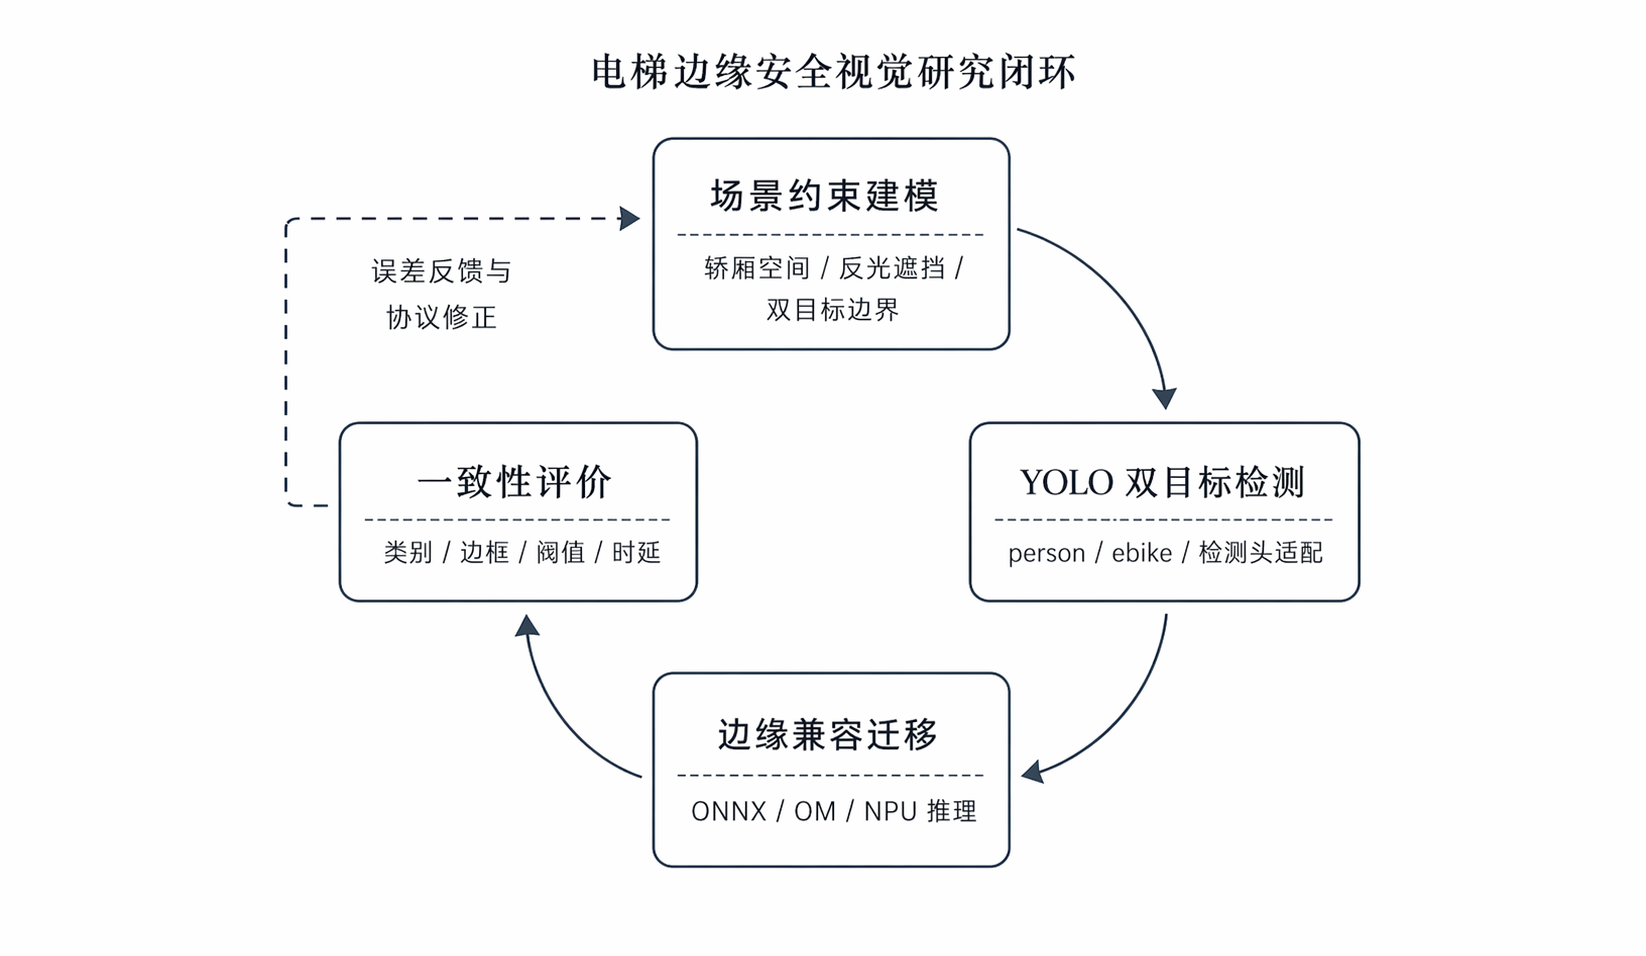
\includegraphics[width=0.92\textwidth]{image/fig1-research-loop.png}
    \caption{本文采用的电梯边缘安全视觉研究流程}
    \label{fig:thesis_loop}
\end{figure}

\section{国内外研究现状}

\subsection{边缘智能与轻量部署方向}

边缘计算的基本思路，是把计算过程尽量放回数据产生的位置附近，以减少传输等待、带宽占用和隐私暴露\cite{shi2016edge,chen2024edgeai}。电梯视频正好具有这几类约束：画面涉及乘客隐私，预警又要求尽快响应，若全部交给云端，网络抖动会直接进入报警链路。围绕端侧运行，模型压缩研究已经给出多种工具。Jacob 等的整数推理友好量化说明，低位宽计算并不必然破坏神经网络性能\cite{jacob2018quantization}；Deep Compression 从剪枝、量化和编码入手压低模型存储与计算成本\cite{han2016deep}；知识蒸馏则提供了把大模型判别能力转移到轻量模型上的常见做法\cite{hinton2015distilling}。

不过，模型真的进入边缘设备后，问题并不止于“文件能不能编译”。训练框架里的浮点权重经过导出、量化或编译后，边框坐标、类别分数排序以及阈值响应都可能发生偏移。离线基准里，这类偏移有时只表现为几个小数点的变化；放到电梯安全视觉中，却可能变成连续画面里的误报、闪烁或漏检。因此，本文关注的不是单次编译成功，而是训练格式、离线模型和板端后处理之间的行为对照\cite{stacker2021deployment,chen2021aqd}。

\subsection{轻量目标检测与实时视觉方向}

实时目标检测已经在工业视觉中形成较成熟的工程路线。YOLO 系列采用端到端预测，结构相对简洁，在不少真实场景中都能直接落地\cite{redmon2017yolo9000}。不同计算预算下，检测网络通常需要在精度和计算量之间取舍：EfficientDet 通过跨尺度特征融合和复合缩放策略取得较好的折中\cite{tan2020efficientdet}；MobileNetV3、EfficientNet 分别从移动端架构搜索和统一缩放规律角度提供了轻量骨干设计参考\cite{howard2019mobilenetv3,tan2019efficientnet}。EdgeYOLO 等工作则把边缘实时检测作为目标，更关注算子友好性、端侧吞吐和推理效率\cite{zhou2023edgeyolo}。

围绕 YOLO 类模型的板端部署，已有研究也开始从算法精度扩展到嵌入式硬件实测。Feng 等在 Jetson Nano、Jetson Xavier NX、Raspberry Pi 4B 与 Intel NCS2 等平台上比较 YOLO 模型的推理流程、帧率和资源占用差异，说明同一检测器在不同边缘设备上会受到计算单元、运行时和模型格式的共同影响\cite{feng2022yolobenchmark}。YOLOBench 进一步在 x86 CPU、ARM CPU、NVIDIA GPU 和 NPU 等嵌入式硬件上评测大量 YOLO 模型，强调模型选择需要结合目标硬件的精度--时延权衡，而不能只依据通用数据集上的离线精度\cite{lazarevich2023yolobench}。这类工作表明，YOLO 边缘部署研究已经从“能否运行”转向“目标硬件上是否具备稳定、可解释的精度和效率表现”。

与上述通用嵌入式平台上的 YOLO 部署基准相比，电梯场景中的双目标检测更强调轻量性、稳定性和板端输出口径一致性。一方面，模型需要识别行人与电动车两个类别，类别数较少，理论上适合轻量模型；另一方面，轿厢内遮挡、反光和近距离尺度变化又会放大轻量模型的表达不足。在前期部署尝试中，YOLOv5 模型在 Hi3516DV500 的 NPU 上占用率可达约 80\%，资源余量有限，后续为追求更好的轻量化效果选择了 YOLOv8n。本文围绕该模型开展部署迁移与一致性评价。

\subsection{困难样本分析与数据增强方向}

当目标检测任务主要受长尾样本和困难样本影响时，单纯扩大数据量并不一定带来稳定收益。OHEM 等在线难例挖掘方法的思路，是让模型把更多训练权重放在当前最容易出错的样本上，从而改善关键失败模式\cite{shrivastava2016ohem}。目标检测中的定向数据增强也有类似作用。Scale-Aware Automatic Augmentation 等研究说明，围绕目标尺度、位置和场景结构设计增强策略，通常比无差别增强更贴近检测误差来源\cite{chen2021scaleaware}。

电梯轿厢中的困难样本具有明显场景规律：反光区域集中在门板和镜面结构，遮挡多发生在人车重叠区域，电动车局部可见常出现在门口或边缘位置。因此，本文将这些因素作为场景复杂性解释工具，用于说明指标变化与实际轿厢结构之间的关系，并将研究重点收束在双目标检测、板端兼容迁移和部署一致性评价上。

\subsection{相关场景研究与当前不足}

与通用监控或道路交通相比，直接面向电梯视觉的公开研究数量并不多。已有工作多聚焦于人数统计、乘客计数或局部行为识别，例如基于 MobileNet-SSD 的电梯人数统计系统研究表明，在电梯场景中采用边缘侧轻量模型是具备现实可行性的\cite{lin2023elevatorcounting}。另一些研究则尝试将轻量模型用于电梯跌倒检测，说明电梯作为独立应用场景具有实际研究价值。

不过，现有研究通常只覆盖单一任务或单一部署环节，较少同时讨论电梯轿厢中的行人与电动车双目标检测、场景复杂性解释以及训练阶段到边缘部署阶段的一致性问题。本文正是在这一不足上展开：以双目标检测为主线，以场景复杂性分析和部署一致性评价为两条支撑线，形成面向电梯安全视觉的研究框架。


\section{研究目标与主要工作}

\subsection{问题定义与核心思路}

从系统角度看，电梯边缘安全视觉不是单独训练一个检测器那么简单。数据来自封闭轿厢，模型要经过导出和编译，还要在开发板应用层完成阈值筛选与 NMS。训练阶段的高精度不能自动说明板端输出仍然可信；反过来，程序能跑起来，也不等于类别、边框和阈值含义没有走样。本文要回答的核心问题是：基于 YOLO 的 \textit{person + ebike} 双目标模型，在 HongOU PI（Hi3516DV500）这样的平台约束下，怎样完成兼容迁移，并用实测指标说明板端输出仍可复查。

这条问题链从轿厢场景本身出发。人车共现、遮挡反光和局部可见，使安全管理需求落到行人与电动车两个类别上；而模型迁移不是简单配置环境，输入尺寸、类别顺序、输出张量和后处理规则都需要逐项核对。本文把 PyTorch 权重、ONNX 中间表示、OM 离线模型以及板端应用后处理放在同一链路中检查。结果分析也采用组合证据：全量验证集说明总体能力，分类别指标暴露行人与电动车差异，阈值、NMS、后处理和分段计时则用来解释板端运行口径。

因此，本文把三个环节连在一起讨论：电梯安全需求被界定为双目标检测任务，模型进入国产边缘平台的过程被写入方法链路，一组可复查实验则用于观察设备端行为。这样处理后，检测精度不再是孤立数字，部署过程也不只是工程背景，而是判断系统能否用于电梯安全视觉的必要证据。

研究动机也来自这个落地过程。电梯安全视觉对漏检和误检都敏感，迁移中的小幅数值变化可能被放大为报警差异。YOLO 检测器虽然部署路径清晰，但输出张量、类别顺序和后处理参数一旦解释错误，板端结果就会偏离训练阶段预期。HongOU PI（Hi3516DV500）开发板采用海思视觉 SoC、专用 NPU 和 OM 离线模型格式，涉及 ONNX 导出、ATC 编译、板端运行时调用和应用层后处理，适合作为本文检查同类目标平台迁移约束的实验载体。

基于这些考虑，论文同时看两件事：模型能否识别行人与电动车，以及模型进入边缘设备后，输出语义和运行口径是否还能对得上训练阶段。只有把这两件事放到同一证据链里，电梯边缘安全视觉系统的可用性才说得清楚。

\subsection{研究目标与主要内容}

本文的研究目标是：面向电梯轿厢中的行人与电动车，完成 YOLO 类双目标检测模型的场景化训练、边缘侧迁移和板端实测分析。具体来说，论文整理从训练权重到 OM 模型再到 HongOU PI（Hi3516DV500）应用输出的检查流程，并用统一实验协议观察检测精度、阈值响应和运行时口径。轿厢中的反光、遮挡和局部可见目标不作为单独创新点展开，而是用于解释误差来源。围绕这一目标，本文完成以下工作。

\begin{enumerate}
    \item 建立电梯轿厢双目标检测任务定义，明确行人与电动车两个核心类别，其中行人检测服务于人员计数与异常感知，电动车检测服务于入梯风险识别。
    \item 总结电梯场景中的典型困难因素，用于解释遮挡、局部可见和光照变化对检测输出的影响。
    \item 分析 YOLO 类检测器在双目标任务中的结构适配方式，说明输入尺寸、类别顺序、检测头输出和 NMS 后处理为什么会影响板端结果。
    \item 梳理从 YOLO 类训练权重、ONNX、OM 到边缘设备执行的迁移链路，检查类别、边框、阈值和运行记录是否能与训练阶段对上。
    \item 基于统一验证集、参数敏感性、后处理消融、代表性片段和分段计时实验，报告总体指标、分类别指标、部署参数影响和边缘设备运行表现。
\end{enumerate}


\subsection{研究难点分析}

本文研究难点并不集中在单一环节。任务层面的困难来自轿厢内行人与电动车经常同时出现，并伴随遮挡、反光、局部可见和尺度变化等问题；模型需要在较小类别集合中保持稳定检测，而不是简单识别静态物体。

模型层面的困难在于，YOLO 类检测器虽然具有较好的实时性，但检测头输出、坐标解码、置信度筛选和 NMS 后处理共同决定最终结果。训练框架脚本通常自动完成这些步骤，而板端应用程序需要显式实现或调用相应逻辑。只要其中一个环节解释不一致，最终输出就可能变化。

部署层面的困难则更接近工程现场。目标平台需要把训练阶段模型转换为可执行的离线模型，并在板端运行时中解释输入、输出和后处理结果。作为本文的实验平台，HongOU PI（Hi3516DV500）开发板具有面向国产边缘 AI 的专用编译和运行时体系，转换过程中的算子适配、预处理配置、数据类型变化和输出读取方式，都会影响设备端行为。因此，部署链路必须进入论文方法本身，而不能只作为实验环境说明。

\subsection{本文的主要工作}

本文工作集中在任务建模、迁移检查和部署评价三个方面。

\begin{enumerate}
    \item \textbf{面向电梯轿厢的双目标检测任务建模。} 本文将电梯安全视觉需求建模为行人与电动车双目标检测问题，行人检测服务于人员计数与拥挤感知，电动车检测服务于入梯风险治理，并用场景复杂性因素解释遮挡、反光和局部可见等因素对检测输出的影响。
    \item \textbf{YOLO 类模型的边缘兼容迁移分析框架。} 本文面向海思/昇腾边缘 AI 平台（以下简称目标平台）及其工具链约束，围绕输入预处理、类别顺序、输出张量、后处理参数和运行时约束整理迁移检查流程，使训练权重、ONNX 中间表示、OM 离线模型和板端应用之间的关键约束能够被逐项检查。
    \item \textbf{面向安全视觉的部署行为对照实践。} 本文不只报告检测精度，还从转换、验证、敏感性、阈值行为和计时等角度分析模型迁移到板端后的实际表现，初步为电梯边缘视觉系统提供一种检查思路。
\end{enumerate}

这些内容分别对应后续章节。任务建模由第一章和第四章承接；迁移检查流程在第三章展开，覆盖输入、类别、输出、后处理和运行五类约束；部署行为对照则由第四章协议和第五章结果共同给出。

\section{研究内容组织逻辑与论文结构}

本文将研究重点放在“模型检测能力”和“边缘部署行为”两个层面。前者说明 YOLO 模型能否在验证集上识别行人与电动车，后者说明模型经过中间表示和离线模型格式进入边缘开发板后，能否继续保持输出含义清楚、结果可以追溯。基于这一思路，第二章介绍 YOLO 和 Hi3516DV500 板端部署基础，第三章给出兼容迁移方法，第四章定义数据、场景复杂性因素和评价协议，第五章基于验证结果分析设备端表现。这样安排后，模型训练、格式转换、设备端运行和实验分析能够串成连续链路。

本文正文共分为五章。第一章介绍研究背景、场景挑战、研究目标和论文结构。第二章回顾目标检测、YOLO 方法、评价指标和 Hi3516DV500 板端部署基础。第三章提出 YOLO 类双目标检测模型的边缘兼容迁移方法。第四章给出数据组织、场景复杂性因素和评测协议。第五章给出实验结果与分析，结论部分总结全文工作并讨论扩展方向。
